\documentclass[a4paper,10pt]{book}
\usepackage[utf8]{inputenc}
\usepackage{tikz}
\usepackage{hyperref}

% simple heading
%   \heading{the text of the heading}
\newcommand{\heading}[1]{
  \vspace{0.3cm} \noindent \textbf{#1} \newline
}

% for inline icons
%   \icon{icon name without path and extension}
\newcommand{\icon}[1]{\tikz[baseline=-3pt] \node[inner sep=0pt,outer sep=0pt]{\includegraphics[height=1.1em]{images/#1}};}

%opening
\title{ADAMS - Scientific Workflow Management}
\author{Peter Reutemann}

\begin{document}

\chapter{Twitter Research}

ADAMS\cite{adams} offers a large amount of actors for a wide range of data processing and data mining tasks. However, we limit ourselves here to the analysis of data obtained from Twitter. The following sections cover how to set up ADAMS in order to access Twitter, how to collect tweets for further (and repeated) analysis, replay previously collected tweets, visualize tweets, use geolocation information and perform some basic text mining.

%%%%%%%%%%%%%%%%%
% Twitter setup %
%%%%%%%%%%%%%%%%%
\section{Twitter setup}
ADAMS uses the twitter4j\footnote{\url{http://twitter4j.org/}{}} library for accessing Twitter. In order to gain access to the Twitter API, you need to have a developer account and register an application to get the required API key/secret and Access token/secret. You can register an application on the Twitter Developer website\footnote{\url{https://dev.twitter.com/}{}} for free. Figure \ref{twitter_dev} shows an example for an ADAMS application, complete with generated API key/secret and Access token/secret. Once you have obtained these keys/tokens/secrets you can enter them in the ADAMS preferences page for Twitter, as shown in Figure \ref{twitter_preferences}. These preferences are global and get picked up by the \icon{TwitterConnection}~TwitterConnection actor as default values, which you can always override, in case you need different credentials.

\begin{figure}[htb]
  \centering
  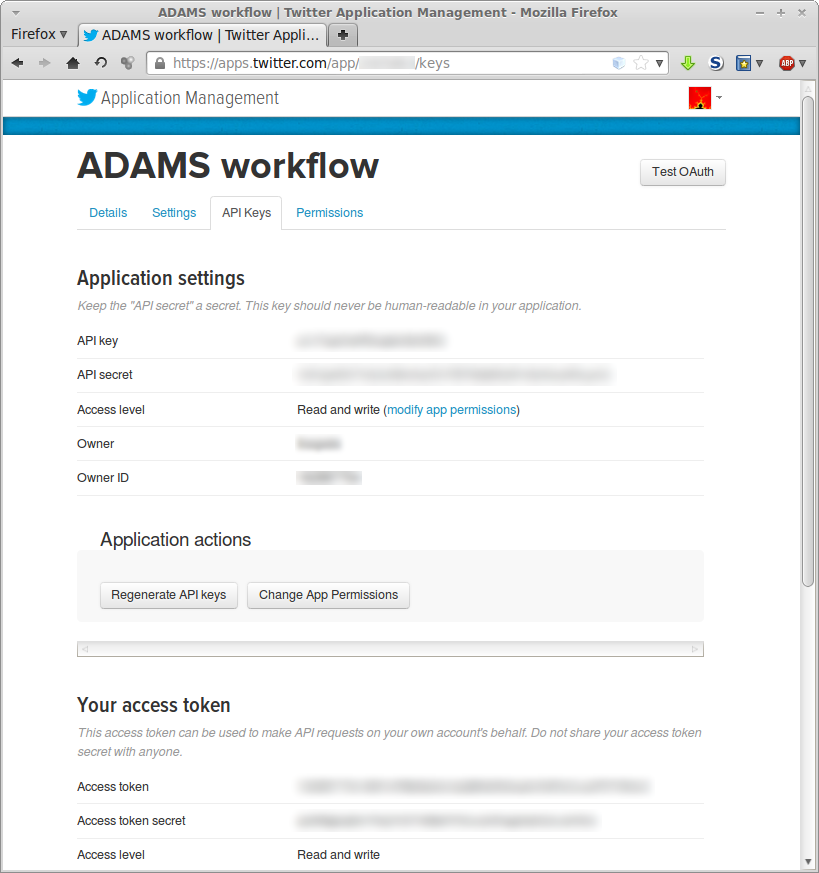
\includegraphics[width=10.0cm]{images/twitter_dev.png}
  \caption{Application management through the ``Twitter Developers'' website, displaying keys, tokens and secrets for an application.}
  \label{twitter_dev}
\end{figure}

\begin{figure}[htb]
  \centering
  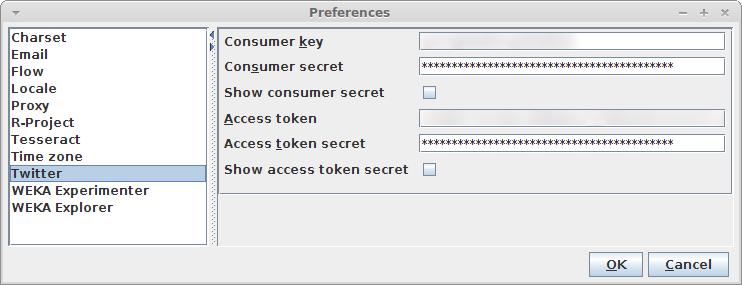
\includegraphics[width=10.0cm]{images/twitter_preferences.png}
  \caption{Preferences page for Twitter in ADAMS.}
  \label{twitter_preferences}
\end{figure}

%%%%%%%%%%%%%%%%%%%%%
% Collecting tweets %
%%%%%%%%%%%%%%%%%%%%%
\clearpage
\newpage
\section{Collecting tweets}
Rather than just obtaining the tweets of a single user, Twitter allows you to tap into the stream of tweets as they are posted in real-time using their streaming API\footnote{\url{https://dev.twitter.com/docs/streaming-apis}{}}. However, Twitter distinguishes between the ``fire hose'' and the ``garden hose''. The former being the complete stream of tweets, which is only accessible to paying customers that have sufficient bandwidth and hardware to cope with the flood of information. The latter is a 1\% sample of the complete stream, which is available to the public. The ``garden hose'' can be accessed using ADAMS.

According to Twitter's API Rules, you can collect tweets, but you are not allowed to redistribute them.\footnote{See \url{https://twitter.com/apirules}{} for more details.} ADAMS therefore fills the void of publicly available tweet archives, by allowing you to collect a large corpus of tweets yourself. You simply set up a flow for collecting tweets and let it run for a number of days, weeks or even months.

\heading{Task}
Collect tweets for future research purposes due to lack of public tweet archives.

\heading{Solution}
In order to collect tweets, you basically only need the following three actors:
\begin{itemize}
  \item \icon{TwitterConnection}~\textbf{TwitterConnection} -- for connecting to Twitter.
  \item \icon{TwitterListener}~\textbf{TwitterListener} -- for accessing the stream of tweets.
  \item \icon{TwitterConverter}~\textbf{TwitterConverter} -- for turning the tweets into a data format suitable for future analysis, e.g., spreadsheet format.
\end{itemize}
Unless you are storing the data in a database, the generated tweet archive file will get rather large, due to several million tweets coming through the ``garden hose'' every single day. The flow depicted in Figure \ref{collect_tweets-flow} saves the tweets in a special ADAMS CSV (comma-separated values) file format, which is also the recommended format for replaying the tweets. In order to avoid too large an output file, the tweets get grouped by day. 

The flow works as follows:
\begin{itemize}
  \item Since we need the file name generation more than once in the flow and we do not want to duplicate the functionality, we push the generation into \icon{CallableActors}~CallableActors, which basically acts as a method call. The file name generation consists of several steps, i.e., we need to encapsulate them in a \icon{SequenceSource}~SequenceSource which we name ``filename''.
  
  \item The \icon{TwitterListener}~TwitterListener source is configured to output an unlimited number of tweets, i.e., the user needs to explicitly stop the flow before the collection process finishes.
  
  \item To begin with, the \icon{Once}~Once control actor\footnote{As the name suggests, the \textit{Once} actor triggers its nested actors only with the first token passing through, as opposed to the default \textit{Trigger} actor which executes its nested actors each time a token passes through.} initializes the variable obtaining the current file name by executing the callable actor ``filename'' through the \icon{CallableSource}~CallableSource source actor and setting the variable \texttt{@\{filename\}} with the \icon{SetVariable}~SetVariable actor.

  \item Every 1000 tweets, the \icon{ConditionalTrigger}~ConditionalTrigger control actor executes its nested actors, checking whether a newly generated CSV file name differs from the one currently stored in the variable \texttt{@\{filename\}}.
    \begin{itemize}
      \item Should that be the case, i.e., the \icon{ConditionalTee}~ConditionalTee actor evaluates to true, the variable \texttt{@\{filename\}} gets updated using the \icon{SetVariable}~SetVariable transformer.
    \end{itemize}
  
  \item Each tweet gets converted into a spreadsheet object using the \icon{TwitterConverter}~TwitterConverter transformer, selecting all data fields deemed important.
  
  \item The generated spreadsheet object then gets stored in the CSV file with the \icon{SpreadSheetFileWriter}~SpreadSheetFileWriter sink, using the current file name stored in the variable \texttt{@\{filename\}}.
\end{itemize}


\begin{figure}[htb]
  \centering
  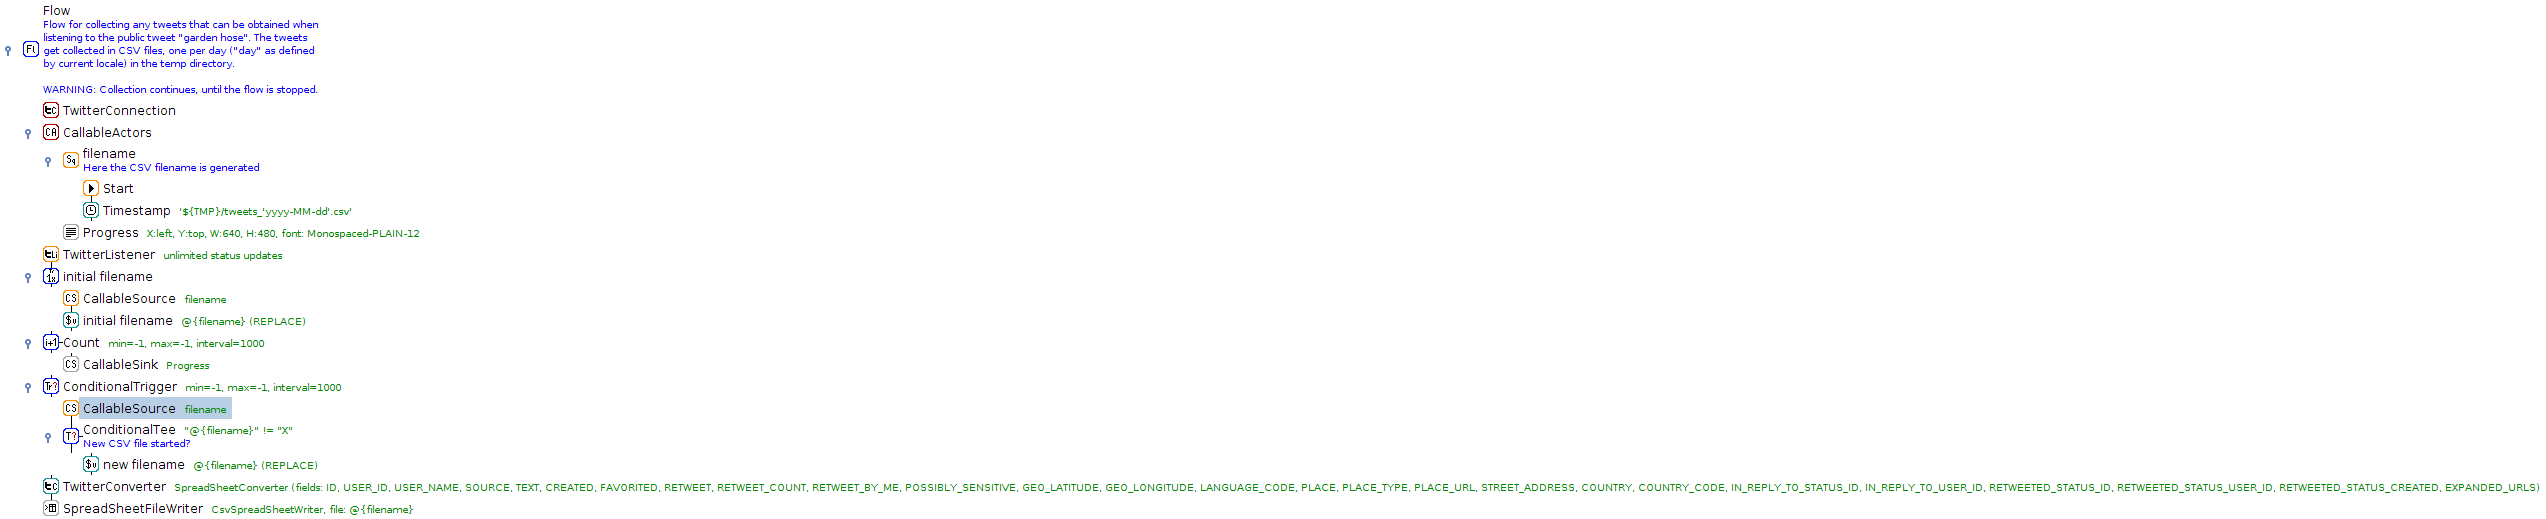
\includegraphics[width=8.0cm]{images/collect_tweets-flow.png}
  \caption{Flow for collecting tweets in CSV archive files.}
  \label{collect_tweets-flow}
\end{figure}

%%%%%%%%%%%%%%%%%%%%%%%%%%%%%%%%%%
% Replaying and filtering tweets %
%%%%%%%%%%%%%%%%%%%%%%%%%%%%%%%%%%
\clearpage
\newpage
\section{Replaying and filtering tweets}
Once you have collected a sufficiently large archive of tweets, you can start experimenting with it. As a first step, we want to demonstrate how you can replay existing archives and how to filter tweets according to user-specified criteria.

\subsection{Basic replay and filtering}

\heading{Task}
Replay tweets from an archive and filter out everything apart from ``happy'' and ``sad'' tweets.

\heading{Solution}
Figure \ref{replay_and_filter_tweets-flow} shows a flow that performs some basic filtering of replayed tweets:

\begin{itemize}
  \item The \icon{TweetReplay}~TweetReplay source replays tweets using the specified tweet replay mechanism, in this case an ADAMS CSV archive.
  
  \item In this case, we want to look into sentiment analysis and therefore only allow tweets that contain a ``happy'' or a ``sad'' smiley. This is done using the \icon{TwitterFilter}~TwitterFilter transformer, which allows you to specify a filter expression. You have access to, if present, the status text, user, language, country, place, ``mentions'', hashtags and GPS location.
  
  \item The \icon{TwitterConverter}~TwitterConverter transformer is used to turn the tweet objects into a textual representation, in this example just the status text.
  
  \item The generated text output is then visualized in a simple text viewer, the \icon{Display}~Display sink.
\end{itemize}

\begin{figure}[htb]
  \centering
  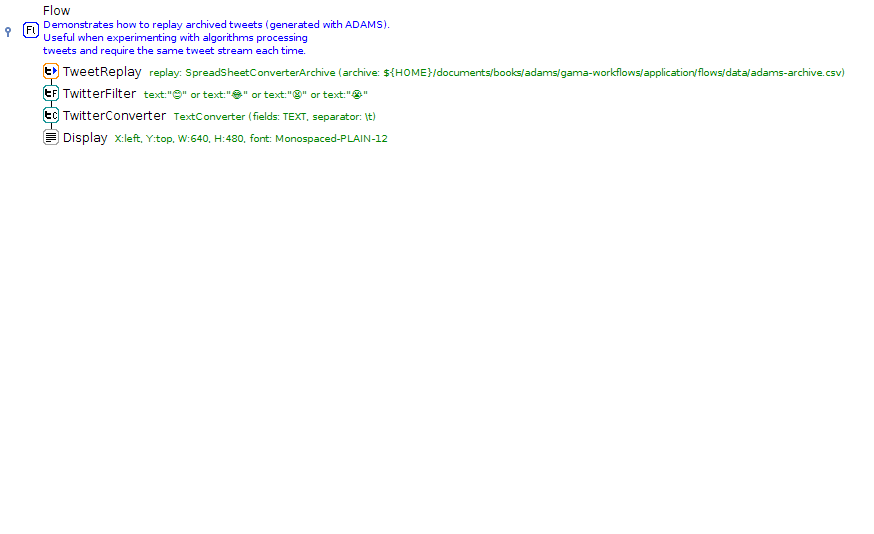
\includegraphics[width=10.0cm]{images/replay_and_filter_tweets-flow.png}
  \caption{Flow for replaying and filtering tweets from a CSV archive, using simple textual output.}
  \label{replay_and_filter_tweets-flow}
\end{figure}

However, if you generated more than one CSV archive, you do not want to manually change the flow each time you want to process another archive file. Using the variable mechanism in ADAMS, you can easily automate the traversal of all the CSV archive files in a directory. Figure \ref{replay_and_filter_tweets-multiple_files-flow} shows how this is done:

\begin{itemize}
  \item With the \icon{DirectoryLister}~DirectoryLister source, you can search directories using a regular expression and output files and/or directories. In our case, we want to output all CSV files (``\texttt{.*\textbackslash.csv}'').
  
  \item The \icon{SetVariable}~SetVariable transformer stores the file names that the \icon{DirectoryLister}~DirectoryLister outputs in the variable \texttt{@\{file\}}.
  
  \item The \icon{Trigger}~Trigger control actor encapsulates now the flow that was introduced in Figure \ref{replay_and_filter_tweets-flow}. However, the ``archive'' option of the SpreadSheetConverterArchive tweet replay mechanism now has the variable \texttt{@\{file\}} attached to it, rather than a fixed file name. This way we will replay one CSV file after the other.
\end{itemize}

\begin{figure}[htb]
  \centering
  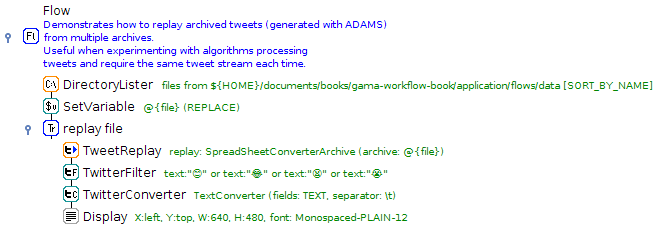
\includegraphics[width=12.0cm]{images/replay_and_filter_tweets-multiple_files-flow.png}
  \caption{Flow for replaying and filtering tweets from multiple CSV archives, using simple textual output.}
  \label{replay_and_filter_tweets-multiple_files-flow}
\end{figure}

\subsection{Plotting calculated values}

Now, simply outputting the status texts of the filtered tweets is not overly interesting, we want to answer some questions with the data that we have collected. For instance, how does the distribution of ``happy'' and ``sad'' smileys change over time?

\heading{Task}
Plot the mood, i.e., ``happy'' and ``sad'' counts, over time.

\heading{Solution}
In order to keep track of the number of tweets in either category, we will use variables to store the counts (per minute in this example). For visualizing, we will use a plotter actor that displays the two curves.

The flow works as follows:
\begin{itemize}
  \item Initialize the \texttt{@\{timetamp\}} variable with an empty string using the \icon{SetVariable-Standalone}~SetVariable standalone.

  \item The \icon{TweetReplay}~TweetReplay source replays a previously generated tweet archive.

  \item In the \icon{Trigger}~Trigger ``determine timestamp'' we determine the timestamp of the current tweet and, if it changed, plot the current counts of happy/sad smileys.
  \begin{itemize}
    \item The \icon{TwitterConverter}~TwitterConverter outputs a ``per minute'' timestamp for the \texttt{CREATED} tweet field.
    \item If \icon{ConditionalTee} ``timestamp changed?'' determines that the new timestamp differs from the old one, we do the following:
    \begin{itemize}
      \item If the \texttt{@\{timestamp\}} variable is not empty, i.e., we have counts for the previous minute available and we want to plot them. This gets determined by the \icon{ConditionalTrigger}~ConditionalTrigger ``plot?''. The actual plotting is explained below.
      \item Record the new timestamp as the current one, using the \icon{SetVariable}~SetVariable actor.
    \end{itemize}
  \end{itemize}
  
  \item The \icon{ConditionalTrigger}~ConditionalTrigger ``happy'' evaluates to true if the twitter text contains a happy smiley and accordingly increments the ``happy'' counter variable using \icon{IncVariable}~IncVariable.
  
  \item The \icon{ConditionalTrigger}~ConditionalTrigger ``sad'' works like the ``happy'' one.
\end{itemize}
The \icon{SequencePlotter}~SequencePlotter sink accepts special ``plot'' containers, which we can generate using the \icon{MakePlotContainer}~MakePlotContainer transformer. This transformer accepts either a single double (``y'') or a double array of length two (``x'' and ``y''). We will generate these plot containers using the timestamp and counts stored in variables, converting them to doubles in the process. Therefore the plotting of the happy/sad counts works as follows (sub-flow beneath the \icon{ConditionalTrigger}~ConditionalTrigger ``plot?''):
\begin{itemize}
  \item In the \icon{Trigger}~Trigger ``timestamp to double'' we are converting the previous ``minute'' timestamp string into milli-seconds (Java epoch) using the \icon{Convert}~Convert transformer in conjunction with the StringToDateTimeType conversion and store the result in the \texttt{@\{timestamp\_double\}} variable.
  
  \item The ``plot happy'' \icon{Trigger}~Trigger then outputs the \texttt{@\{timestamp\_double\}} and \texttt{@\{happy\}} variables as string array, converts it to a double array using the \icon{ArrayProcess}~ArrayProcess control actor with the nested \icon{Convert}~Convert actor (using the StringToDouble conversion), creates a plot container using the \icon{MakePlotContainer}~MakePlotContainer transformer (labeled ``happy'') and feeds it into the call-able \icon{SequencePlotter}~SequencePlotter sink using the \icon{CallableSink}~CallableSink actor.
  
  \item The ``plot sad'' sub-flow works the same way.
  
  \item The \icon{SetVariable}~SetVariable transformers ``reset happy'' and ``reset sad'' reset the counters to 0 for the next minute.
\end{itemize}
Figure \ref{replay_and_filter_tweets2-output} shows the generated plot from a small tweet archive that spans only a few minutes. Apart from the fact that people seem to post more ``happy'' smileys, not much else can be gleaned from this plot.

However, when we aggregate the counts over hours rather than minutes, it is possible to see trends much better. Figure \ref{twitter_mood} shows the smiley distribution over New Years 2013/14\footnote{In the early hours of the new year, a network outage prohibited the collection of tweets.}. You can clearly see that the ``sad'' smileys follow closely the ``happy'' ones, though at a reduced rate. But around the changeover of years, the counts for the ``happy'' smileys skyrocket before settling back to a more normal level. The second, smaller ``happy'' bump later in the day on New Years Day is probably due to people getting up and replying to tweets that they received the night before.

\begin{figure}[htb]
  \centering
  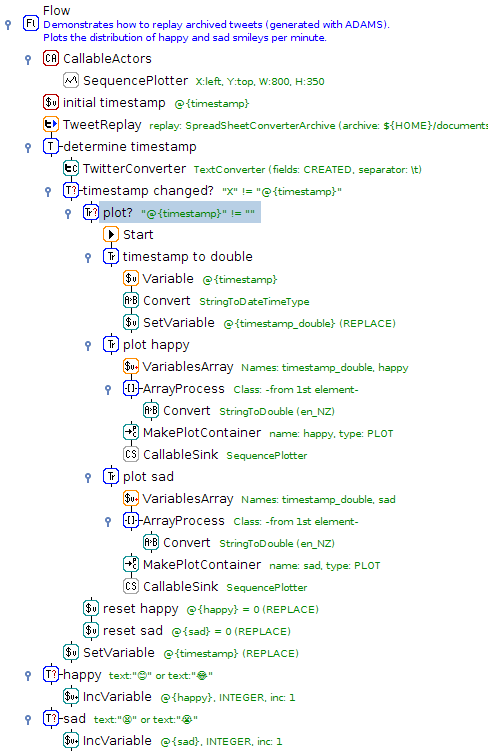
\includegraphics[width=8.0cm]{images/replay_and_filter_tweets2-flow.png}
  \caption{Flow for replaying and filtering tweets from a CSV archive, displaying mood distribution per minute.}
  \label{replay_and_filter_tweets2-flow}
\end{figure}

\begin{figure}[htb]
  \centering
  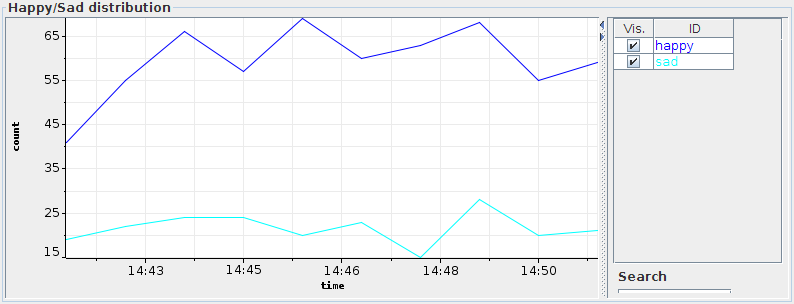
\includegraphics[width=10.0cm]{images/replay_and_filter_tweets2-output.png}
  \caption{Visualization of mood distribution per minute (``happy'' and ``sad'' smiley counts).}
  \label{replay_and_filter_tweets2-output}
\end{figure}

\begin{figure}[htb]
  \centering
  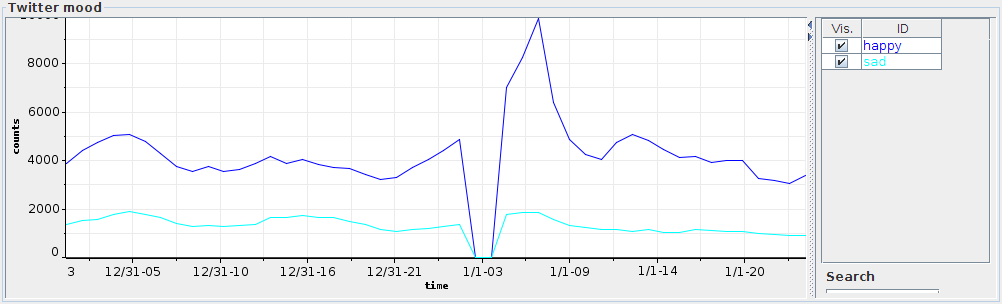
\includegraphics[width=12.0cm]{images/twitter_mood.png}
  \caption{Visualization of mood distribution per hour over New Years 2013/2014 (``happy'' and ``sad'' smiley counts).}
  \label{twitter_mood}
\end{figure}

%%%%%%%%%%%%%%%
% Geolocation %
%%%%%%%%%%%%%%%
\clearpage
\newpage
\section{Geolocation}
Twitter enables users to attach their geolocation\footnote{WikiPedia on geolocation: \url{https://en.wikipedia.org/wiki/Geolocation}{}} in the form of GPS coordinates to the tweets that they are sending. In the previous section, we discovered how to analyze tweets along the time axis. Using the geolocation information of tweets in conjunction with the OpenStreetMap\footnote{\url{http://www.openstreetmap.org/}{}} support available in ADAMS, we can visualize tweets on a map over time. The visualization can either be generated from a tweet archive (see Figure \ref{visualize_tweets-archive-flow}) or in real-time (see Figure \ref{visualize_tweets-realtime-flow}), by listening to the tweets as they occur. The archive approach is much faster, as ADAMS can usually process tweets faster than they become available through Twitter's ``garden hose''.

The spreadsheet data structure in ADAMS allows you not only to represent primitives such as boolean, long, double, string and various date types, you can also store arbitrary objects. These objects get converted to and from strings using handlers that are registered for specific data types. GPS coordinates conversion is one application of this generic functionality. Displaying geolocation data therefore first converts the GPS coordinates obtained from the tweets into GPS objects before generating special map objects to be displayed on the map itself.

\heading{Task}
Display tweets with geolocation information on a map of the world.

\heading{Solution}
The flow for displaying the geolocation tweets is relatively simple:
\begin{itemize}
  \item The tweets get generated once again using the \icon{TweetReplay}~TweetReplay source.
  
  \item Since we require geolocation information, we filter the tweets with a \icon{TwitterFilter}~TwitterFilter transformer, that ensures that latitude and longitude values are present.
  
  \item A \icon{ConditionalTee}~ConditionalTee with a TwitterFilterExpression is used to check for ``happy'' tweets. In case of such a tweet, a ``layer'' name for the map and the associated ``color'' of the marker on the map are set using \icon{SetVariable}~SetVariable actors. The tweet is then sent off to be plotted on the map using the \icon{CallableSink}~CallableSink actor, referencing the \icon{Sequence}~Sequence actor ``TweetMap''. This control actor encapsulates the following steps:
  \begin{itemize}
    \item In order to have a notion of the time passing when the tweet archive is processed, the \icon{OpenStreetMapViewer}~OpenStreetMapViewer sink ability to displayed overlays on the map can be used to display the current value of a variable. Therefore we set the variable \texttt{@\{timestamp\}} with the timestamp generated from the \texttt{CREATED} field of the tweet inside the \icon{Tee}~Tee actor ``create timestamp for overlay'' and use this variable in the overlay ``TextMapOverlay'' of the map set up.
    
    \item Before we can convert the GPS coordinates into objects, we need to combine the two column in the generated tweet spreadsheet into a single one using the SpreadSheetJoinColumns conversion in the \icon{Convert}~Convert transformer ``join long/lat''.
    
    \item The newly created GPS column can then be turned into GPS objects using the SpreadSheetStringColumnToObject conversion, \icon{Convert}~``gps'', with a handler for processing GPS coordinates.
    
    \item The final conversion, \icon{Convert}~``map objects'', then turns the GPS objects into marker objects suitable for the map (SpreadSheetToMapObjects).
    
    \item The map objects get channeled into the \icon{OpenStreetMapViewer} map sink itself. Since we do not want to accumulate all the tweets in the map, but rather want to provide a ``mood'' window, we define a pruning strategy in the map. Since our tweet archive covers only a short period, we use a simple pruning strategy that removes all  map objects that are at least two minutes older than the newest map object.
  \end{itemize}

  \item Processing of ``sad'' smileys works accordingly, but with different layer name and color.
\end{itemize}
In Figure \ref{visualize_tweets-archive-output} you can see the final display of tweets from the archive with the timestamp overlay of ``2014-02-12 14:52'' in the top-right corner. ``Happy'' tweets are colored in green and ``sad'' ones in red. Left-clicking with the mouse on one of the map markers brings up the associated information, in this case tweet status text, tweet date and GPS coordinates.

\begin{figure}[htb]
  \centering
  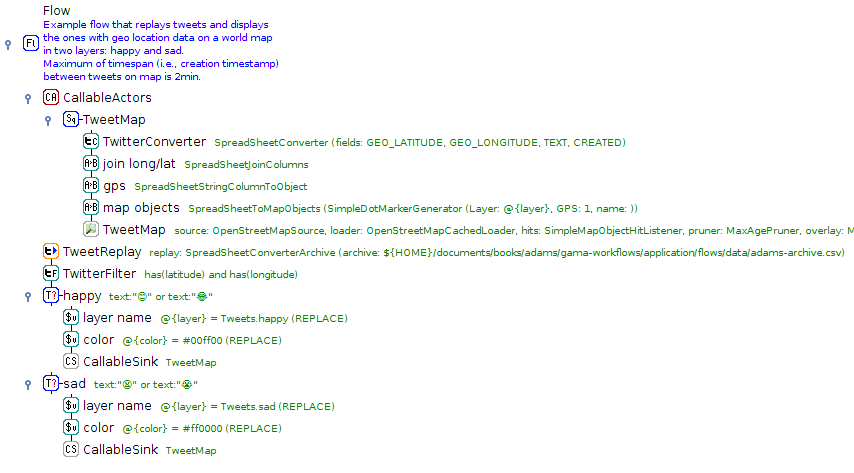
\includegraphics[width=12.0cm]{images/visualize_tweets-archive-flow.png}
  \caption{Flow for visualizing tweets with geolocation information.}
  \label{visualize_tweets-archive-flow}
\end{figure}

\begin{figure}[htb]
  \centering
  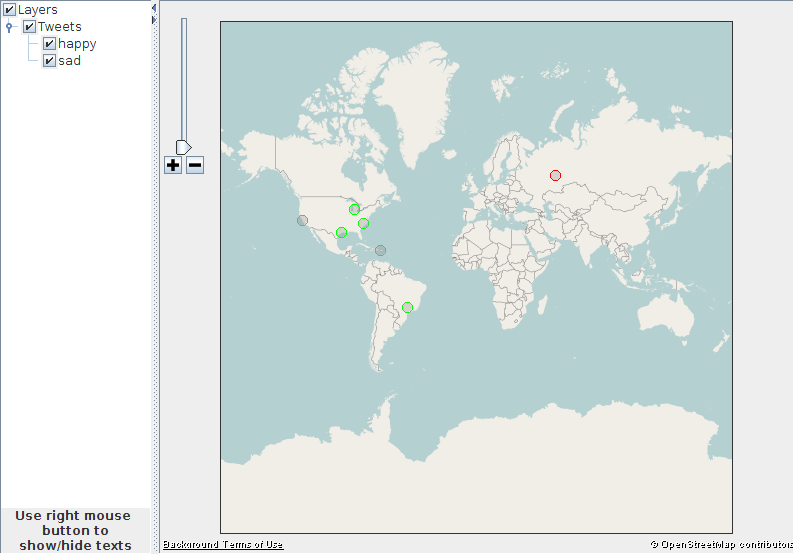
\includegraphics[width=10.0cm]{images/visualize_tweets-archive-output.png}
  \caption{Visualization of tweets with geolocation information.}
  \label{visualize_tweets-archive-output}
\end{figure}

\begin{figure}[htb]
  \centering
  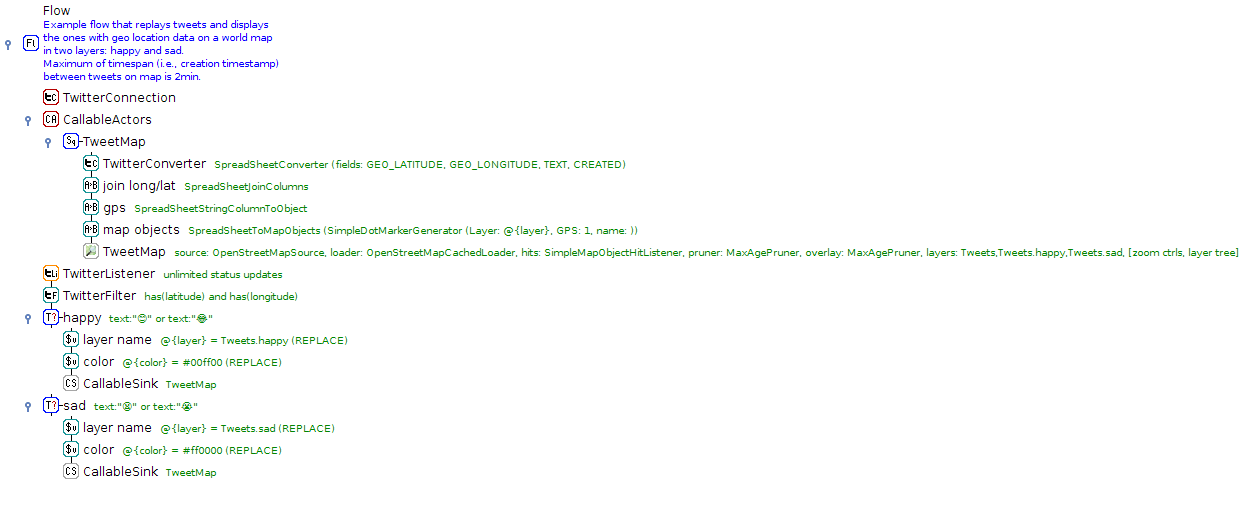
\includegraphics[width=12.0cm]{images/visualize_tweets-realtime-flow.png}
  \caption{Flow for visualizing geolocation tweets in real-time.}
  \label{visualize_tweets-realtime-flow}
\end{figure}

%%%%%%%%%%%%%%%
% Text mining %
%%%%%%%%%%%%%%%
\clearpage
\newpage
\section{Text mining}
So far we have covered how to collect tweet data and perform some visualizations. In this section you will see how you can apply data mining techniques, i.e., Weka\cite{weka} algorithms, to your data archives.

\subsection{Converting the data}
Before we can evaluate data mining algorithms on our collected data, we need to convert it into a format that Weka can handle. The simplest approach is to create a combined CSV file in the specific format that Weka is able to load\footnote{Weka escapes quotes with a backslash rather than doubling them up as most office packages do. It also turns tabs, new lines, carriage returns into \textbackslash t, \textbackslash n and \textbackslash r respectively.}.

\heading{Task}
Combine multiple data archives into single dataset that Weka can read.

\heading{Solution}
With Weka we have the choice of either creating a CSV file that can be read by Weka's CSVLoader or creating a native ARFF file. The CSV file approach has the advantage that we can always ``append'' more data to it. Using an ARFF file, on the other hand, is more efficient in regards to I/O. In the following we will describe two flows that cover both scenarios.
The first flow, depicted in Figure \ref{csv_archive_to_weka_csv-flow}, copies all the content of all the CSV archive files that the user choses into a single Weka CSV file:
\begin{itemize}
  \item The \icon{SetVariable-Standalone}~SetVariable standalone defines the file name for the combined CSV file. It gets stored in the user's temporary directory, under the name \texttt{combined.csv}.

  \item Inside the \icon{Trigger}~Trigger ``convert csv'' the CSV conversion takes place:
  \begin{itemize}
    \item With the \icon{SelectFile}~SelectFile source, we limit the user to selecting CSV files. All of the selected files will get combined. The current file name gets stored with the \icon{SetVariable}~SetVariable actor in \texttt{@\{input}\}.
    
    \item Below the \icon{Trigger}~Trigger ``convert'' we convert the CSV archives into the Weka format:
    \begin{itemize}
      \item We attach the variable \texttt{@\{input}\} to the ``archive'' parameter inside the \icon{TweetReplay}~TweetReplay source.
      
      \item With \icon{TwitterConverter}~TwitterConverter with once again turn the tweet object into a spreadsheet representation.
      
      \item The \icon{SpreadSheetFileWriter}~SpreadSheetFileWriter sink then appends the spreadsheet row generated from the tweet in a Weka-compatible CSV format.
    \end{itemize}
  \end{itemize}

  \item The \icon{Trigger}~Trigger ``output csv filename'' merely outputs the absolute file name of the CSV file that was generated.
\end{itemize}

\begin{figure}[htb]
  \centering
  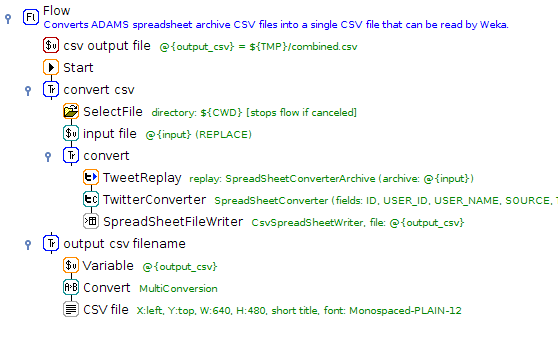
\includegraphics[width=12.0cm]{images/csv_archive_to_weka_csv-flow.png}
  \caption{Turning tweets archives into single Weka CSV file.}
  \label{csv_archive_to_weka_csv-flow}
\end{figure}

The second flow, depicted in Figure \ref{csv_archive_to_arff-flow}, creates a single Weka ARFF file from all the CSV archive files that the user choses, ready for text mining. Furthermore, it filters out all tweets that are neither ``happy'' nor ``sad'' and creates a dataset with two attributes, one with the text of the tweet and a class attribute with the labels, ``happy'' or ``sad'':
\begin{itemize}
  \item In addition to the CSV output variable, the \icon{SetVariable-Standalone}~SetVariable standalone defines the file name for the final ARFF file. It gets stored in the user's temporary directory, under the name \texttt{combined.arff}.

  \item The \icon{Trigger}~Trigger ``convert csv'' the CSV conversion takes place, similar to the one in the previous flow (Figure \ref{csv_archive_to_weka_csv-flow}). However, between the \icon{TweetReplay}~TweetReplay source and the \icon{SpreadSheetFileWriter}~SpreadSheetFileWriter sink, additional filtering and a different conversion takes place:
  \begin{itemize}
    \item The \icon{TwitterFilter}~TwitterFilter only lets ``happy'' and ``sad'' tweets through.
    
    \item We initialize the variable \texttt{@\{class\}} with a missing value ``?'', using the \icon{SetVariable}~SetVariable actor.
    
    \item The \icon{ConditionalTee}~ConditionalTee actors, ``happy'' and ``sad'', set the variable \texttt{@\{class\}} accordingly, either ``happy'' or ``sad''.
    
    \item Since we only want to mine the status text of tweets, the \icon{TwitterConverter}~TwitterConverter only turns the \texttt{TEXT} field into a spreadsheet object, i.e., one with only a single column.
    
    \item Now we need to introduce a new column for the class attribute, using the \icon{SpreadSheetInsertColumn}~SpreadSheetInsertColumn transformer.
    
    \item With the \icon{SpreadSheetSetCell}~SpreadSheetSetCell actor we set the class label using the value stored in the variable \texttt{@\{class\}}, before writing it to disk using the \icon{SpreadSheetFileWriter}~SpreadSheetFileWriter.
  \end{itemize}
  
  \item Inside the \icon{Trigger}~Trigger ``convert to arff'', we load the combined CSV file and turn it into an ARFF file, as the name suggests:
  \begin{itemize}
    \item The \icon{FileSupplier}~FileSupplier source outputs the file name stored in the variable \texttt{@\{output\_csv\}}.
    
    \item With the \icon{WekaFileReader}~WekaFileReader, configured to use a specific CSVLoader setup, we turn the CSV file into a Weka dataset.
    
    \item We then push the dataset through the \icon{WekaFilter}~WekaFilter transformer, to turn the class attribute from type \texttt{STRING} to \texttt{NOMINAL}.
    
    \item Finally, we save the dataset under the file name stored in \texttt{@\{output\_arff\}}, using the \icon{WekaFileWriter} sink.
  \end{itemize}
  
  \item The \icon{Trigger}~Trigger ``output arff filename'' merely displays the full file name of the generated Weka dataset, like in the previous flow.
\end{itemize}


\begin{figure}[htb]
  \centering
  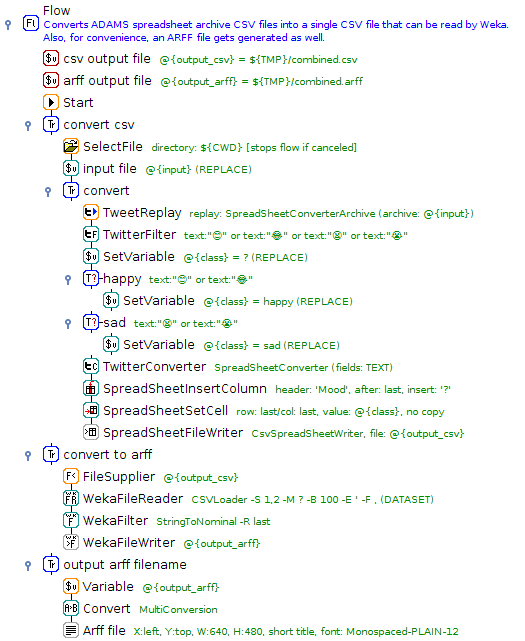
\includegraphics[width=10.0cm]{images/csv_archive_to_arff-flow.png}
  \caption{Turning tweets archives into single Weka ARFF file.}
  \label{csv_archive_to_arff-flow}
\end{figure}

\subsection{Evaluating the data}
Once the data has been turned into a format for Weka, we can then apply text mining techniques. Most classification algorithms are not able to work with text data directly, but need some form of transformation. We will use the StringToWordVector filter available in Weka for exactly this reason. Though it offers many parameters, we will only use it with default parameters. As for the classifier, we will use J48, Weka's implementation of Quinlan's C4.5\cite{c45}.

\heading{Task}
Cross-validate the J48 algorithm on the ``mood'' dataset.

\heading{Solution}
As basis for our flow, we will use the flow introduced earlier for turning the CSV file archives into a single ARFF file (see \ref{csv_archive_to_arff-flow}). But we will skip the step on saving the dataset as ARFF file, since we can work with the in-memory dataset itself:
\begin{itemize}
  \item The \icon{Trigger}~``evaluate'' trigger, starts with the same steps of loading the data from CSV, namely \icon{FileSupplier}~FileSupplier, \icon{WekaFileReader}~WekaFileReader and \icon{WekaFilter}~WekaFilter.
  
  \item Since we are now dealing with a classification task, we need to define which attribute is the class attribute (``last''). We achieve this by using the \icon{WekaClassSelector}~WekaClassSelector actor.
  
  \item The cross-validation on the dataset is performed by the \icon{WekaCrossValidationEvaluator}~WekaCrossValidationEvaluator actor. However, this actor does not list the classifier setup explicit, instead it points to a ``call-able'' actor\footnote{By moving the classifier setup to a ``callable'' actor we can re-use the same setup in multiple places (e.g., evaluation and model generation), without having to worry about changing it in multiple places. Also, the setup does not have to be generated by a WekaClassifierSetup actor, but can be loaded from a serialized model or generated from a command-line representation.}, which we have to supply. This is done with the \icon{WekaClassifierSetup}~WekaClassifierSetup source at the top of the flow, which is configured with J48 and StringToWordVector wrapped using Weka's FilteredClassifier meta-classifier. We do not want to display any classifier errors, hence we can discard the predictions and conserve memory.
  
  \item In order to turn the container, that the cross-validation actor outputs, into human-readable output, we can either pick specific statistics or simply output a summary. We do the latter here using the \icon{WekaEvaluationSummary}~WekaEvaluationSummary actor, inlcuding ``confusion matrix`` and ``class details`` in the output.
  
  \item The generated summary is then displayed in the \icon{Display}~Display sink. An example output is shown in Figure \ref{crossvalidate_csv_archive-output}.
\end{itemize}


\begin{figure}[htb]
  \centering
  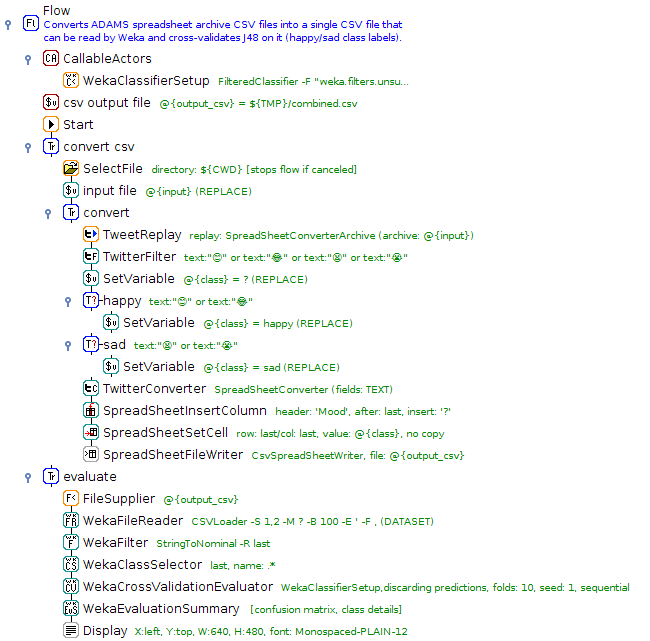
\includegraphics[width=12.0cm]{images/crossvalidate_csv_archive-flow.png}
  \caption{Cross-validating ``mood'' of tweets archives using J48.}
  \label{crossvalidate_csv_archive-flow}
\end{figure}

\begin{figure}[htb]
  \centering
  {\scriptsize
  \begin{verbatim}
=== Summary ===

Correctly Classified Instances         611               76.2797 %
Incorrectly Classified Instances       190               23.7203 %
Kappa statistic                          0.3153
Mean absolute error                      0.2733
Root mean squared error                  0.4042
Relative absolute error                 67.9764 %
Root relative squared error             90.1795 %
Coverage of cases (0.95 level)          98.2522 %
Mean rel. region size (0.95 level)      76.5918 %
Total Number of Instances              801     


=== Confusion Matrix ===

   a   b   <-- classified as
  78 145 |   a = sad
  45 533 |   b = happy


=== Detailed Accuracy By Class ===

                 TP Rate  FP Rate  Precision  Recall   F-Measure  MCC      ROC Area  PRC Area  Class
                 0.350    0.078    0.634      0.350    0.451      0.338    ?         ?         sad
                 0.922    0.650    0.786      0.922    0.849      0.338    ?         ?         happy
Weighted Avg.    0.763    0.491    0.744      0.763    0.738      0.338    0.000     0.000     
  \end{verbatim}}
  \caption{Results of cross-validating ``mood''.}
  \label{crossvalidate_csv_archive-output}
\end{figure}

\begin{thebibliography}{999}
	% to make the bibliography appear in the TOC
	\addcontentsline{toc}{chapter}{Bibliography}

	\bibitem{adams}
		Reutemann, Peter and Vanschoren, Joaquin (2012); 
		\textit{Scientific Workflow Management with ADAMS};
		In Peter A. Flach, Tijl Bie, and Nello Cristianini, editors, 
		Machine Learning and Knowledge Discovery in Databases, 
		volume 7524 of Lecture Notes in Computer Science, pages 
		833-837; Springer Berlin Heidelberg.
		
	\bibitem{weka}
	    Mark Hall, Eibe Frank, Geoffrey Holmes, Bernhard Pfahringer, Peter 
	    Reutemann, Ian H. Witten (2009); \textit{The WEKA Data Mining Software: An 
	    Update}; SIGKDD Explorations, Volume 11, Issue 1.
	    
	\bibitem{c45}
	    Ross Quinlan (1993); \textit{C4.5: Programs for Machine Learning}; 
	    Morgan Kaufmann Publishers, San Mateo, CA.

\end{thebibliography}

\end{document}
